\documentclass{standalone}
\usepackage{tikz}
\usetikzlibrary{arrows.meta, positioning, shapes.geometric, fit, backgrounds, calc, shadows, decorations.pathmorphing}
\usepackage{xcolor}
\usepackage{amsmath}
\usepackage{amssymb}

% Define colors
\definecolor{AbstractColor}{RGB}{70, 130, 180}    % Steel Blue for abstract concepts
\definecolor{FunctionalColor}{RGB}{60, 179, 113}  % Medium Sea Green for functional concepts
\definecolor{ComputationalColor}{RGB}{221, 160, 221} % Plum for computational concepts
\definecolor{AIColor}{RGB}{255, 165, 0}          % Orange for AI learning concepts
\definecolor{ConnectorColor}{RGB}{105, 105, 105}  % Dim Grey for connectors

\newcommand{\E}{\mathcal{E}}
\newcommand{\elder}[1]{\E^{#1}}
\newcommand{\eldersubspace}{\E_{\text{elder}}}
\newcommand{\mentorsubspace}{\E_{\text{mentor}}}
\newcommand{\eruditesubspace}{\E_{\text{erudite}}}

\begin{document}
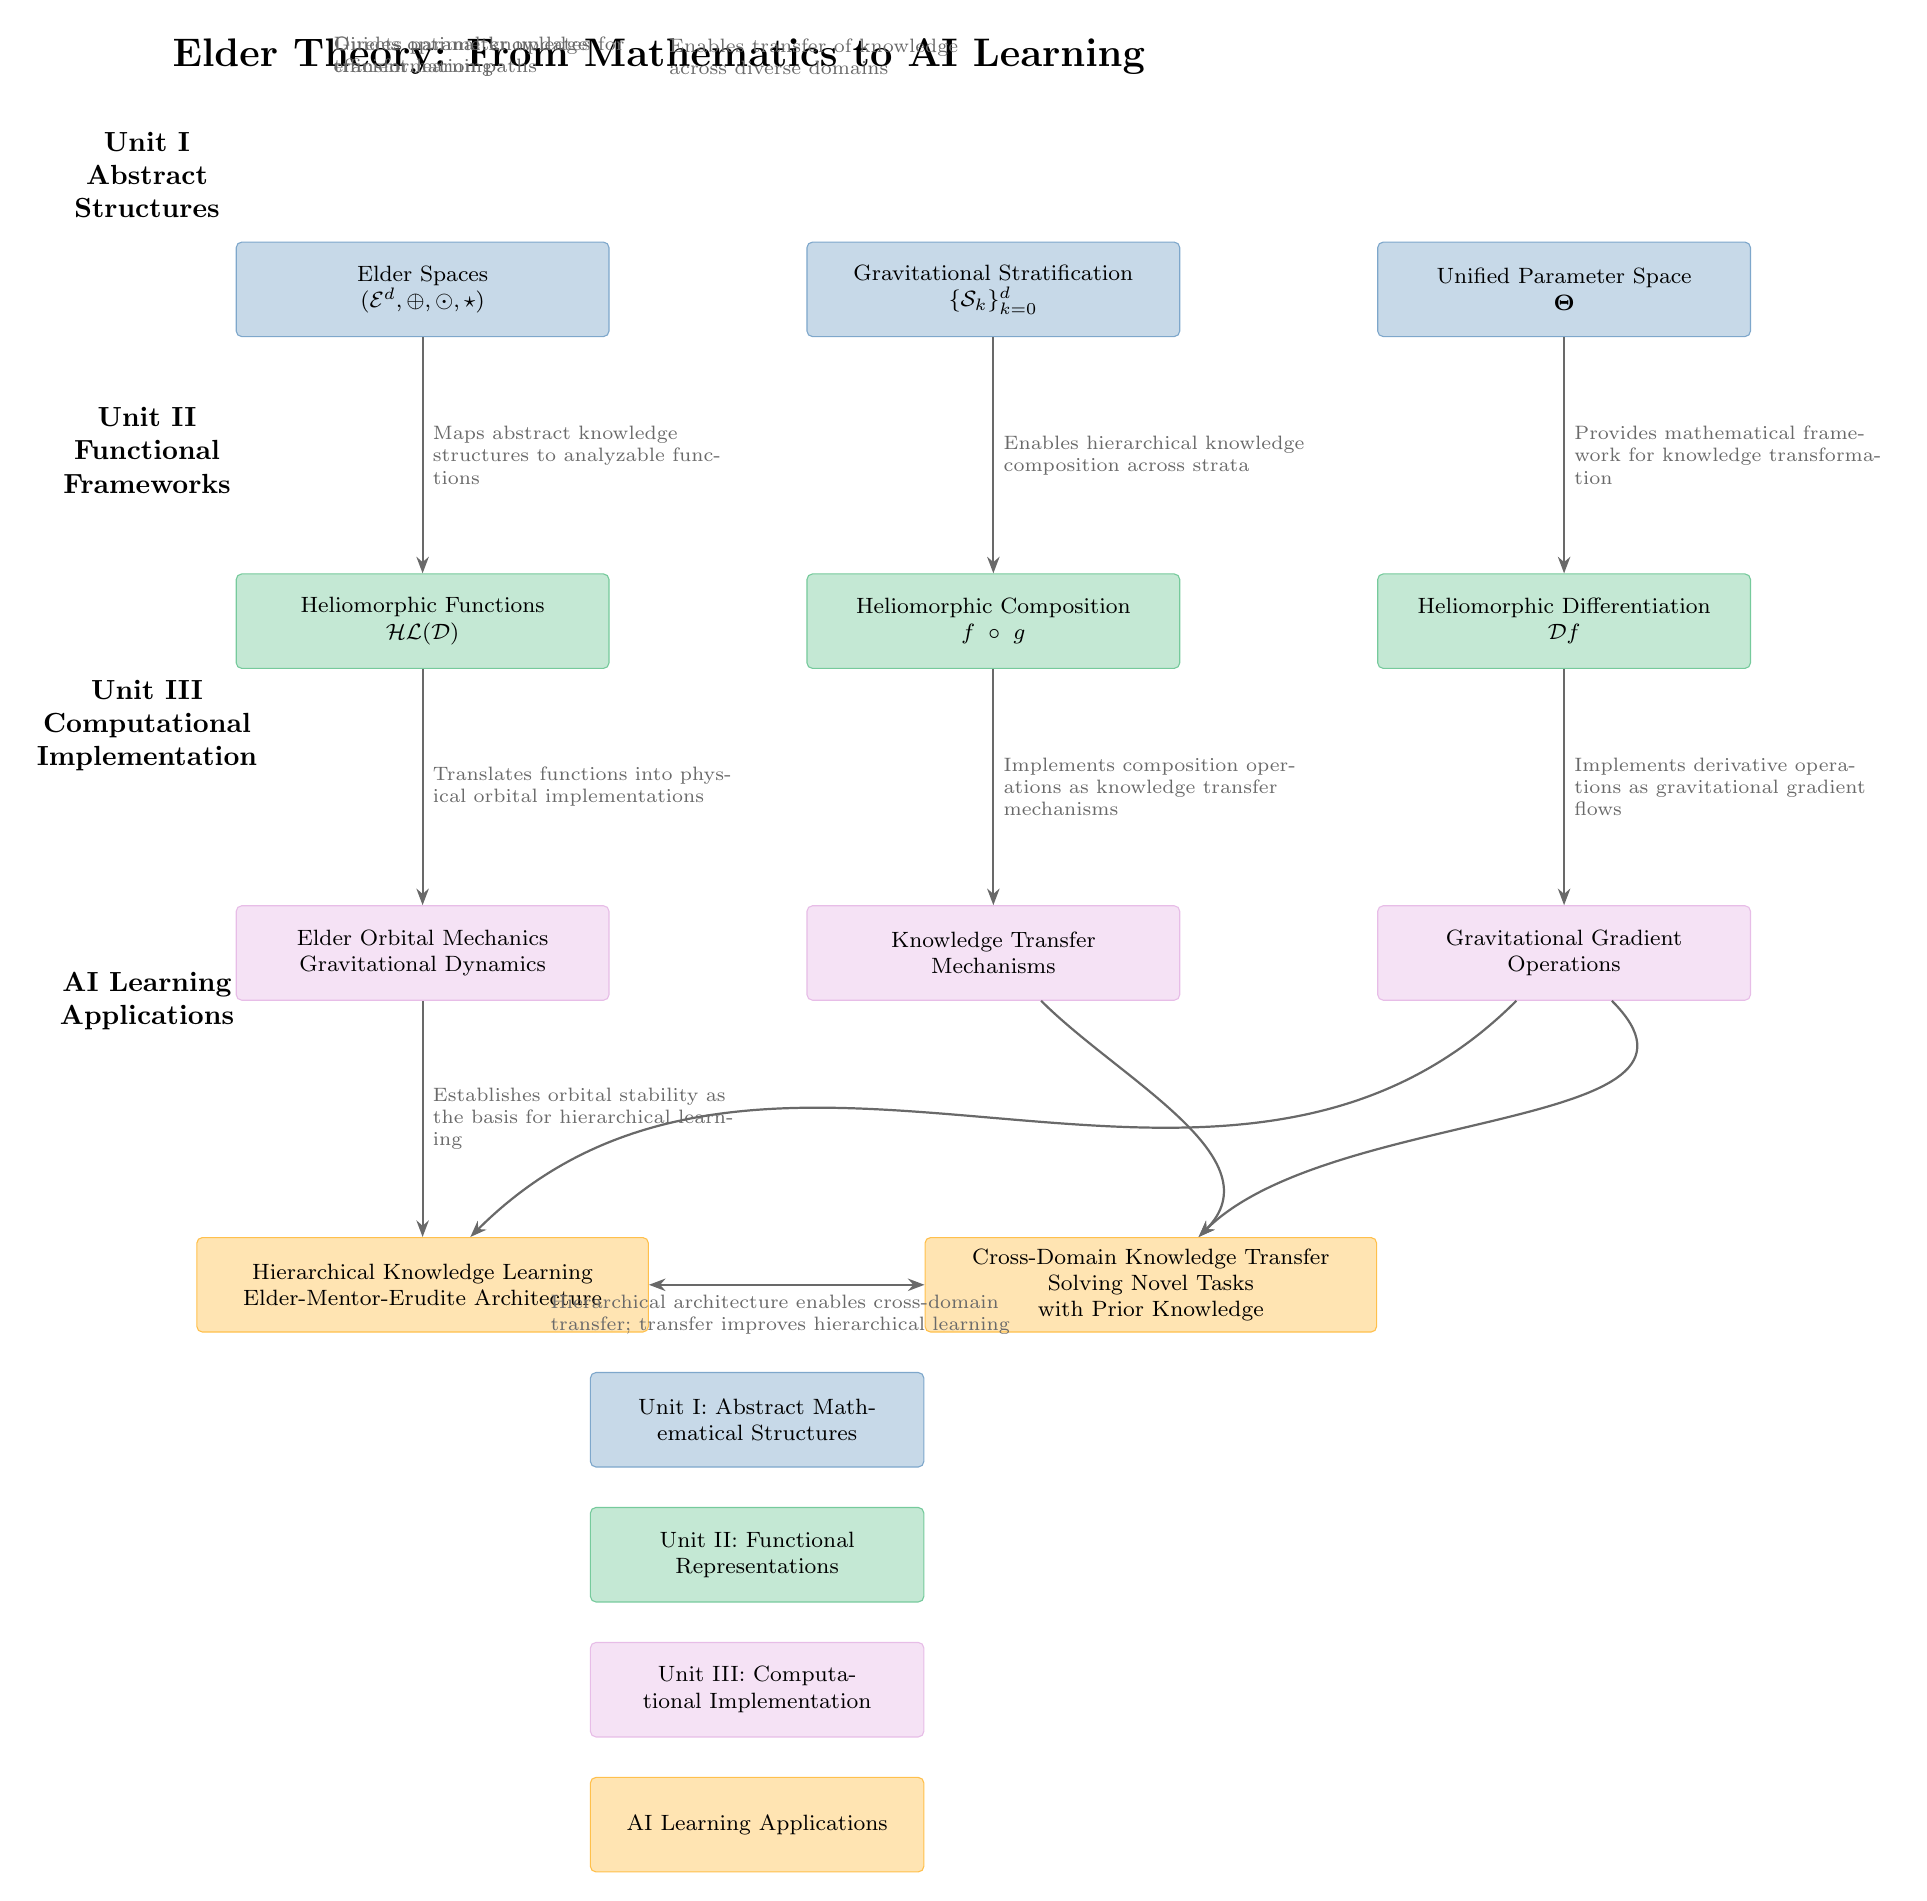
\begin{tikzpicture}[
    node distance=2.5cm and 2.5cm,
    box/.style={
        draw, 
        rounded corners=2pt, 
        text width=4.5cm, 
        minimum height=1.2cm,
        align=center,
        font=\footnotesize
    },
    abstract/.style={box, fill=AbstractColor!30, draw=AbstractColor!70},
    functional/.style={box, fill=FunctionalColor!30, draw=FunctionalColor!70},
    computational/.style={box, fill=ComputationalColor!30, draw=ComputationalColor!70},
    ai/.style={box, fill=AIColor!30, draw=AIColor!70, text width=5.5cm},
    arrow/.style={-{Stealth[length=6pt]}, thick, ConnectorColor},
    doublearrow/.style={{Stealth[length=6pt]}-{Stealth[length=6pt]}, thick, ConnectorColor},
    title/.style={font=\Large\bfseries},
    subtitle/.style={font=\large\bfseries, align=center},
    layer/.style={font=\bfseries, align=center}
]

% Title
\node[title] at (0, 0) (title) {Elder Theory: From Mathematics to AI Learning};

% Unit levels
\node[layer] at (-6.5, -1.5) {Unit I\\Abstract\\Structures};
\node[layer] at (-6.5, -5) {Unit II\\Functional\\Frameworks};
\node[layer] at (-6.5, -8.5) {Unit III\\Computational\\Implementation};
\node[layer] at (-6.5, -12) {AI Learning\\Applications};

% Abstract Mathematical Structures (Unit I)
\node[abstract, below=2cm of title, xshift=-3cm] (elder_spaces) {Elder Spaces \\ $(\elder{d}, \oplus, \odot, \star)$};
\node[abstract, right=of elder_spaces] (gravitational_stratification) {Gravitational Stratification \\ $\{\mathcal{S}_k\}_{k=0}^d$};
\node[abstract, right=of gravitational_stratification] (parameter_space) {Unified Parameter Space \\ $\boldsymbol{\Theta}$};

% Functional Representations (Unit II)
\node[functional, below=3cm of elder_spaces] (heliomorphic_functions) {Heliomorphic Functions \\ $\mathcal{HL}(\mathcal{D})$};
\node[functional, right=of heliomorphic_functions] (heliomorphic_composition) {Heliomorphic Composition \\ $f \circ g$};
\node[functional, right=of heliomorphic_composition] (heliomorphic_differentiation) {Heliomorphic Differentiation \\ $\mathcal{D}f$};

% Computational Implementation (Unit III)
\node[computational, below=3cm of heliomorphic_functions] (orbital_mechanics) {Elder Orbital Mechanics \\ Gravitational Dynamics};
\node[computational, right=of orbital_mechanics] (knowledge_transfer) {Knowledge Transfer \\ Mechanisms};
\node[computational, right=of knowledge_transfer] (gradient_operations) {Gravitational Gradient \\ Operations};

% AI Learning Applications
\node[ai, below=3cm of orbital_mechanics] (hierarchical_learning) {Hierarchical Knowledge Learning \\ Elder-Mentor-Erudite Architecture};
\node[ai, below=3cm of knowledge_transfer, xshift=2cm] (cross_domain_transfer) {Cross-Domain Knowledge Transfer \\ Solving Novel Tasks with Prior Knowledge};

% Connections from Abstract to Functional
\draw[arrow] (elder_spaces) -- (heliomorphic_functions) 
    node[midway, right, text width=3.8cm, font=\scriptsize] {Maps abstract knowledge structures to analyzable functions};
\draw[arrow] (gravitational_stratification) -- (heliomorphic_composition)
    node[midway, right, text width=4cm, font=\scriptsize] {Enables hierarchical knowledge composition across strata};
\draw[arrow] (parameter_space) -- (heliomorphic_differentiation)
    node[midway, right, text width=4cm, font=\scriptsize] {Provides mathematical framework for knowledge transformation};

% Connections from Functional to Computational
\draw[arrow] (heliomorphic_functions) -- (orbital_mechanics)
    node[midway, right, text width=3.8cm, font=\scriptsize] {Translates functions into physical orbital implementations};
\draw[arrow] (heliomorphic_composition) -- (knowledge_transfer)
    node[midway, right, text width=4cm, font=\scriptsize] {Implements composition operations as knowledge transfer mechanisms};
\draw[arrow] (heliomorphic_differentiation) -- (gradient_operations)
    node[midway, right, text width=4cm, font=\scriptsize] {Implements derivative operations as gravitational gradient flows};

% Connections from Computational to AI Applications
\draw[arrow] (orbital_mechanics) -- (hierarchical_learning)
    node[midway, right, text width=4cm, font=\scriptsize] {Establishes orbital stability as the basis for hierarchical learning};
\draw[arrow] (knowledge_transfer) to[out=-45, in=45] (cross_domain_transfer)
    node[midway, right, text width=4cm, font=\scriptsize] {Enables transfer of knowledge across diverse domains};
\draw[arrow] (gradient_operations) to[out=-45, in=45] (cross_domain_transfer)
    node[pos=0.7, left, text width=4cm, font=\scriptsize] {Guides optimal knowledge transformation paths};
\draw[arrow] (gradient_operations) to[out=-135, in=45] (hierarchical_learning)
    node[pos=0.7, left, text width=4cm, font=\scriptsize] {Directs parameter updates for efficient learning};

% Horizontal connections
\draw[doublearrow] (hierarchical_learning) -- (cross_domain_transfer)
    node[midway, below, text width=6cm, font=\scriptsize] {Hierarchical architecture enables cross-domain transfer; transfer improves hierarchical learning};

% Legend
\node[abstract, text width=4cm, below=0.5cm of cross_domain_transfer, xshift=-5cm] (leg1) {Unit I: Abstract Mathematical Structures};
\node[functional, text width=4cm, below=0.5cm of leg1] (leg2) {Unit II: Functional Representations};
\node[computational, text width=4cm, below=0.5cm of leg2] (leg3) {Unit III: Computational Implementation};
\node[ai, text width=4cm, below=0.5cm of leg3] (leg4) {AI Learning Applications};

\end{tikzpicture}
\end{document}